%%%%%%%%%%%%%%%%%%%%%%%%%%%%%%%%%%%%%%%%%%%%%%%%%%%%%%%%%%%%%%%%%%%
%                                                                 %
%                            CHAPTER TWO                          %
%                                                                 %
%%%%%%%%%%%%%%%%%%%%%%%%%%%%%%%%%%%%%%%%%%%%%%%%%%%%%%%%%%%%%%%%%%%

\chapter{LITERATURE REVIEW}\label{ch:prevwork}
%\resetfootnote %this command starts footnote numbering with 1 again.

\section{Introduction}

The data versioning landscape produces a variety of different approaches and standards towards change capture.
However, massive centralized data stores have become more prevalent as data distribution methods advance  \cite{Vassiliadis1999}.
Collection into larger unified repositories will likely require a multi-tiered approach to synchronize the varied practices  \cite{Baker2009}.
Baker notes that differences depend on the sociotechnical distance of a repository from the data's origin \cite{Baker2009}.
Local stores closer to the collection site better understand data capture conditions, but must also adapt to changing environments.
Science agencies and organizations are only beginning to formally codify and standardize methods to capture and publish lineage information \cite{MatthewS.Mayernik201312-039}.
This seems to be a recurring cycle of attention with rapidly developing technologies such as the grid or parallel computing \cite{Kovse2003VGridAVS}.
The CERN grid for the Compact Muon Solenoid experiment carefully developed necessary processes which allow references by multiple users to the same file without copying that file across the grid \cite{Holtman:687353}.

The model defined in Chapter \ref{ch:model} provides a basis for understanding the formal underlying properties which will allow consistent versioning practices.
Previous work in provenance, provenance distance, and mapping provide inspiration for the model's form.
A majority of the linked data approaches to version capture can be found in provenance models.
Additionally, researchers have attempted to address the amount of change between version identifiers using a measure called provenance distance.
This distance measure lacks sufficient resolution to provide detailed quantities to answer many versioning questions.
The model also draws inspiration from existing change mapping methods found in version control managers to reduce space consumption when working with large data sets.
These mapping methods provide a familiar and regularized basis to both compute and present changes.

\section{Data Versioning Operations}

Versioning systems come in a variety of different forms as a result of the assorted applications they must manage.
Experimental biology data require tracking as they pass through a scientific workflow \cite{Tagger2005}.
Libraries curate multiple editions of the same work, sometimes with significant revisions \cite{Wiil:2000:RDH:338407.338517}.
What such activities demonstrate is the wide range of settings and expectations under which versioning systems operate.
While this work cannot hope to explore all these applications, every system studied shares three common functions: addition, deletion, and modification.
These three operations plausibly form the core set of relationships when versioning.

Literature surveys often expect versioning systems to interact with data uniformly because they are asked to perform the same functions \cite{Tagger2005}.
However, different data sets may utilize each of the three core operations at different rates \cite{rohtua}.
This helps to characterize the data set in ways such as a growing set with many additions, a stable collection featuring occasional corrections, or a wildly volatile data set consisting of often deleted and replaced data files.
Understanding these would give insight into the maturity and health of a data set, but most major provenance ontologies do not heavily feature these relationships.
Versioning information, of course, does not give insight into the origins of an object, and therefore, would not be expected to play a major role in provenance documentation.

While data addition and modification remain fairly uncontroversial, there is a mild division between practical and theoretical approaches to data deletion \cite{Flouris04clotho:transparent}.
A removed object provides evidence of an erroneous activity's results or intermediary steps leading to a final product.
As a result, version management should maintain and track invalidated data.
The software versioning manager GIT uses a method of compressing older data to conserve space without deleting the data \cite{Chacon:2009:PG:1618548}.
Available storage space places pragmatic constraints on the number of projects which can adopt snapshotting practices.
In applications which cannot recover erroneous data nor use it as documentation artifacts, like corrupted surveillance images.
Some high energy physics experiments cannot re-collect observational data due to cost, and as a result, they cannot replace or re-process poor quality data \cite{Cavanaugh2002}.
While the distinction between `deletion' and `invalidations' remains largely semantic, the terms' use in this document reflects an understanding of the different constraints and requirements placed on versioning systems.
As a result, invalidation is adopted as a broad, general term to also encompass data deletions.

A handful of other operations exist among version managers, but they do not prove ubiquitous across most applications.
Software versioning tools like RCS commonly feature branching and merging functions to create a versioning line separate from the stable master branch \cite{tichy1985rcs}.
This mostly provides an organizational role in development by allowing developers to experiment without contaminating a stable software release.
Figure \ref{GITTree} models this, showing versions C3 and C5 in branch iss53 before being merged back into the production line as C6.
It allows for more orderly management of versions, but does not conduct versioning itself.
Other activities provide functional operations such as locking and unlocking files from edits to prevent race conditions in branch mergers.
It does not introduce any new relationships but allows the tool to operate more smoothly.
Clotho, a versioning application managing versions at the block level, coordinates constrained spaces using intermittent compact and un-compact methods when retrieving or storing old objects \cite{Flouris04clotho:transparent}.
Likewise, many version control tools include functions to display the versioning tree, but this is also an ease-of-use function \cite{Dijkstra1994}.

\begin{figure}
	\centering
	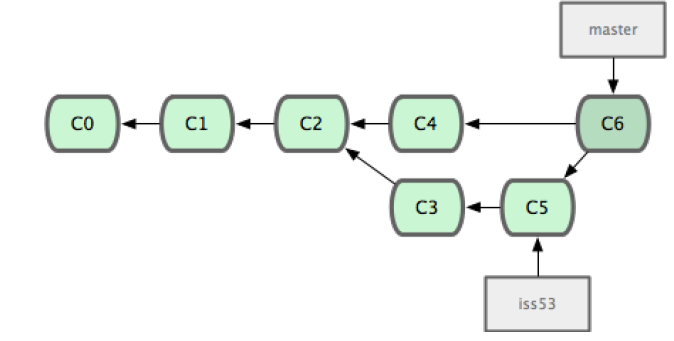
\includegraphics[scale=0.75]{figures/GITCommitTree.png}
	\caption[Example of a commit history with branching stored in GIT.]{Example of a commit history with branching stored in GIT.  Figure 3.17 from \cite{Chacon:2009:PG:1618548}}
	\label{GITTree}
\end{figure}

\subsection{Types of Change}

Barkstrom uses the ability to scientifically distinguish between two data sets as a criteria for major divisions among groupings \cite{Barkstrom2003}.
At lower levels, he notes that science teams can no longer discern scientific differences between data sets.
Instead, they observe that changes to format and structure contribute significant alterations without changing any values withing the data.
As a result, these technical changes form a second boundary to meaningfully separate minor version groupings.
Finally, the explicit values may need occasional revisions to correct lexical errors such as spelling or formatting.
These terms were chosen carefully as they reflect the three value dot-decimal identifier system.
However, data producers will often use qualitative measures to determine the type of change occurring between versions.
Versioning system users wish to achieve insight into the type of change that occurs between versions, and quantitative analysis on versioning operations will provide quantifiable evidence in characterizing the impact of a change.

The exact category that a particular change falls into can be controversial.
The decision to provide concentration units from parts per million to milligrams per milliliter poses a Technical change for a data producer.
However, for a data consumer, the alteration may be viewed as a Scientific change as it invalidates the methods they had previously used.
This conflict in view illustrates the data consumer-producer dynamic.
In general, data producers control the versioning methods, but data consumers determine the classification of a data change.
Producers tend to use versioning systems to ensure data quality of service through audits and recovery tools \cite{Cavanaugh2002}.
Meanwhile, a consumer will analyze the historical changes and determine the impact this may have on their data use.
As a result, this means that data versioning systems must communicate a dynamic view of the changes in a system contextualized by the user of that data.

Version managers often disagree at the point many technical changes sufficiently modifies a data set that it comprises a scientific change.
As determining changes in science requires expert understanding over a domain, different measures should be explored to address the distinction.
This document's approach studies add, invalidate, and modify counts to quantify the impact of changes and how they relate to the producer's observations.
As previously mentioned, different systems utilize the operations at varying rates so absolute cutoffs will be unlikely in comparison to relative results.

\section{Identifiers}

Data managers often impose a sequential ordering in conjunction with logical groupings to form an object's historical lineage \cite{barkstrom2014earth}.
As a result, they often employ version identifiers in the dot-decimal style where a decimal point connects together a series of numbers \cite{Stuckenholz:2005:CEV:1039174.1039197}.
Whenever, a new version is made, it receives an identifier with one of the numbers incremented as seen in Figure \ref{RCSTree}.
Changes to the left-most number often signify a more important change.
Many software applications use the 3-number Major.minor.revision format in labeling software releases.
Numbering the version this way, however, does allow computers and readers to quickly parse the version name and discern that a change has occurred, but not much value exists beyond that \cite{Dijkstra1994}.
Most importantly, it groups together changes from the lower spectrum of minor or major change with those in the upper, more impactful, changes.
It is, therefore, difficult to obtain a clear characterization of a version change without a longer series of numbers.
This method of identification also has issues since small changes in the current data set may have larger implications for data farther down the workflow, which is not communicated by the identifier.
In addition, version numbers capture the overall change of a data set, but users may not interact with collections that way.
Data on a hurricane sometimes occupy only a small portion of a data set, and the files may not even be adjacent in the collection \cite{Barkstrom_digitallibrary}.
There is also little standardization or formal requirements in naming methods.
Ubuntu utilizes a dot-decimal version labeling scheme where the two number identifier corresponds to the year-month values of the release \cite{Ubuntu}.
Fischer, et al., demonstrate the importance of having a regular standardized version identification system, as it provides a mechanism to track errors being addressed \cite{Fischer2003}.
The ability to link bug reports and versions thus gives producers and customers metrics to understand how developers fix errors and how long it will take.
A common method used to address the distinction between versions is a human-readable change log, further discussed in Section \ref{sec:changelog}.


\begin{figure}
	\centering
	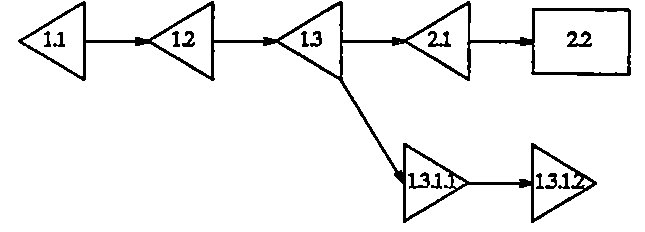
\includegraphics[scale=0.75]{figures/RCSCommitTree.png}
	\caption[Commit history of an object in RCS with changes in the main line stored as back deltas and side branches stored as forward deltas.]{Commit history of an object in RCS with changes in the main line stored as back deltas and side branches stored as forward deltas.  Figure 5 in \cite{tichy1985rcs}}
	\label{RCSTree}
\end{figure}

In many ways, versioned objects resemble multi-edition books or documents.
Digital librarians have faced many challenges when searching for an identifier due to evolving web technologies.
Early citations referred to on-line documents using stagnant Uniform Resource Locators (URL), but this frequently lead to a condition known as link rot where moving the document would invalidate the URL \cite{Lyons2005}.
Locators required a system to manage changes of old identifiers to new locations when people attempted to utilize references from print.
This eventually led to the development of Persistent URLs (PURL), which also suffered from link rot, and this eventually led to the distributed Digital Object Identifier (DOI) system used to track documents today \cite{Duerr2011}.
The PURL used a centralized system that would translate dead links and redirect to a document's latest location.
However, the system would still need to be manually updated, meaning links would rot if a document was lost or overlooked.
DOIs rely on a network of managing agencies to collect and host submitted documents.
In the specialized Handle system, the network has member agencies internally assign an unique name and concatenate it to the end of their host name.
In Figure \ref{table:Duerr}, DOIs represent the most suitable identifier used for citation in scholarly literature \cite{Duerr2011}.
The DOI network provides a robust system to track documents, but when tracking data, it faces difficulty following the rate of change with more volatile data sets.
Under current definitions, distribution organizations assign different DOIs to separate editions of a document.
Documents often do not need new identifiers since they change very rarely as a result of the publication process.
However, the data set production and distribution cycle moves more quickly and reacts more sensitively to small content changes, including when data collection continues on after initial publication.
This behavior becomes entirely too slow as data providers begin allowing users to dynamically generate data products from existing data according to their needs \cite{Barkstrom2003a}.
Some agencies have begun assigning versioned DOIs, but this has not become common practice.
Other groups do not assign a new DOI, but reference to the latest release of the document or object \cite{Ands2017}.
As data sets continue to grow in size, it may become impractical to look towards data as the driving source for identifiers, as Proell and Rauber suggest that database queries may provide a more scalable means of citing data sets \cite{proellBigData}.

\begin{figure}
	\centering
	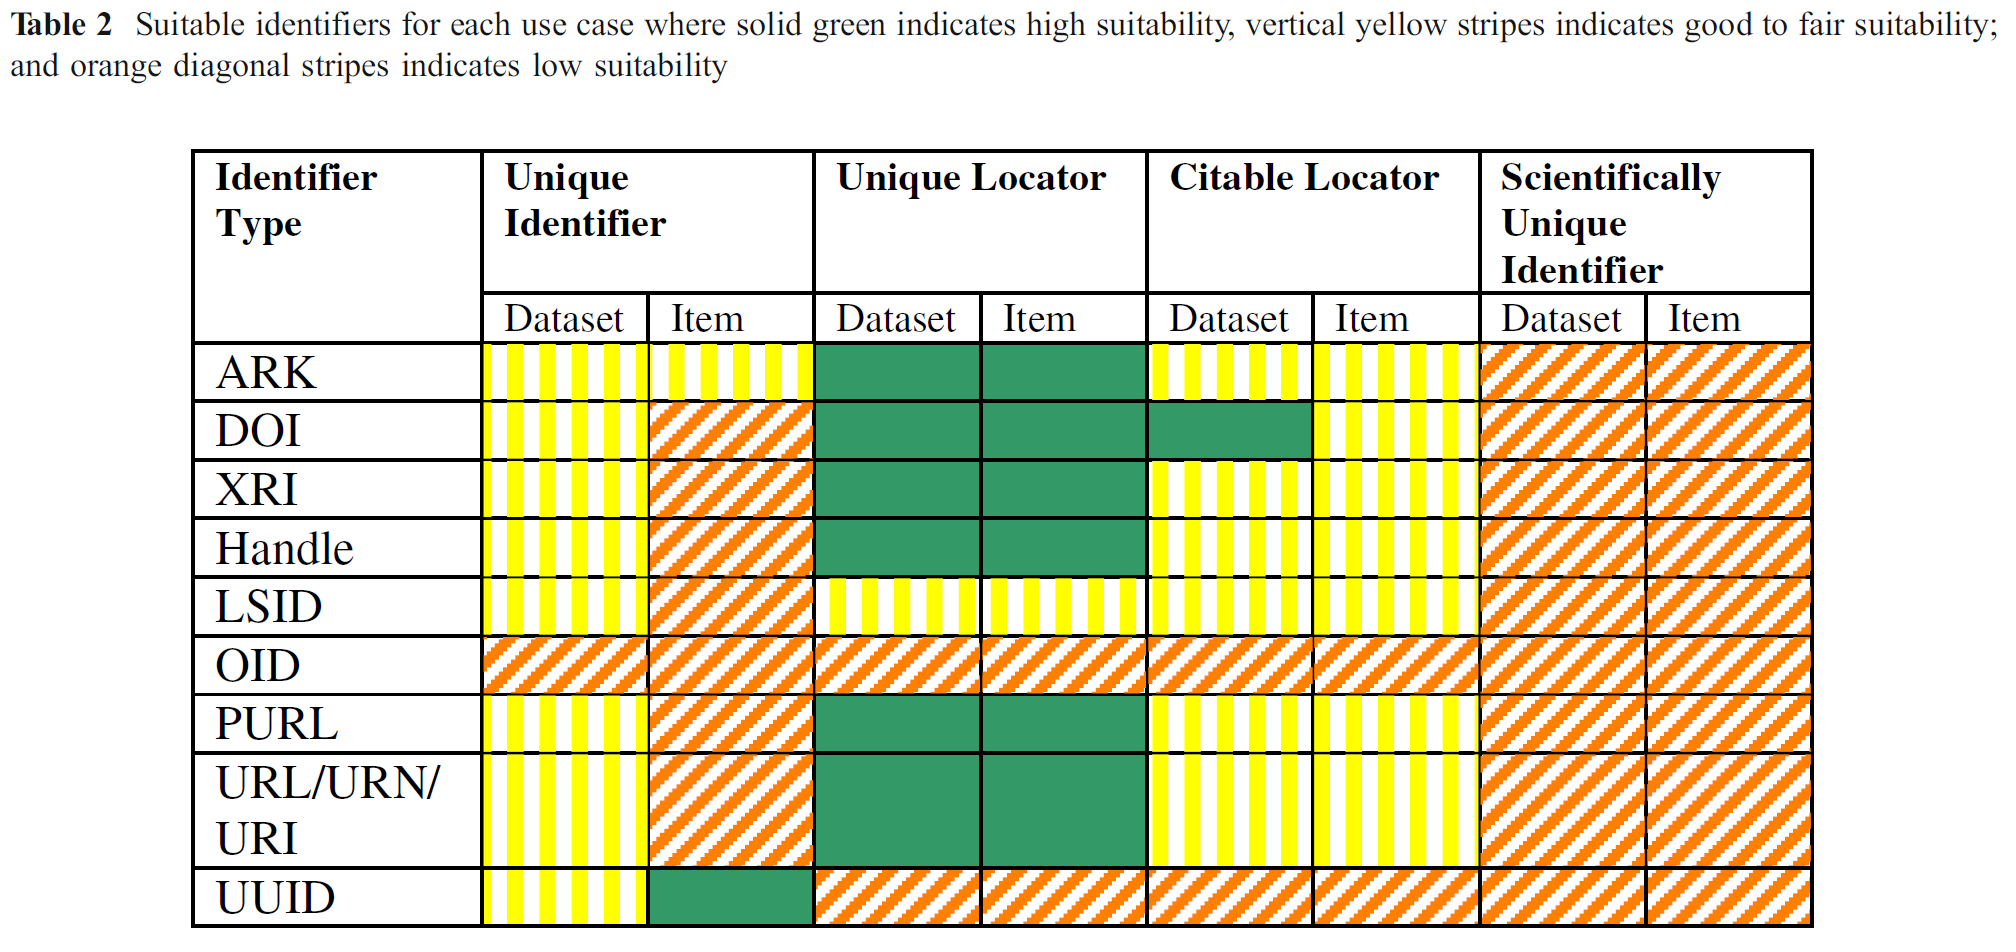
\includegraphics[scale=0.30]{figures/DigitalIdentifierTable.png}
	\caption[Table of predominant identifiers used in science.]{Table of predominant identifiers used in science.  From Duerr, et al. \cite{Duerr2011}}
	\label{table:Duerr}
\end{figure}

The discourse on DOIs highlights the importance of understanding the limitations of particular identifier schemes.
With respect to Figure \ref{table:Duerr}, no identification scheme fits the description of a scientific identifier.
Duerr, et al., define a use case to make the argument that scientifically unique identifiers are necessary, ``to be able to tell that two data instances contain the same information even if the formats are different" \cite{Duerr2011}.
A possibility to consider is that identifiers may require incorporation into a data model to discern between scientific differences.
An identifier works well in revealing the characteristics of an individual object, but it should not be expected to explain its relationship with other objects.
A data model provides better insight into the different roles objects play in a relationship.
Further discussion on versioning models will be found in Section \ref{sec:models}.
This proves increasingly important as the ability to propagate relevant data change across autonomous systems then assures valid quality in interactions between domains \cite{Systems02champagne:data}.

Using identifiers to convey extended versioning information becomes more difficult with the adoption of distributed version managers like GIT \cite{cederqvist2002version}.
Each participant in the federated repository is the master of their personal copy of the code.
Upon completion of their distribution's part, they may request that it be pulled into another participant's distribution.
While each developer's individual repository can follow a linear identifier scheme, this would not work as the overall project bounces around different primary repositories with mismatching sequential identifiers.
The dot-decimal identifier scheme could be made to work in such an environment by severely limiting the distributed manager's utilized features.
Figure \ref{fig:federated} illustrates a workflow which utilizes distributed repositories to manage very active public software projects.
Each lieutenant developer manages a section of the overall code, and they dampen the number of requests made to the dictator by collecting changes and submitting them over longer intervals.
As a result, relying on identifiers to convey and contain versioning information limits the evolution of new and valuable methods of processing change in digital objects.

\begin{figure}
	\centering
	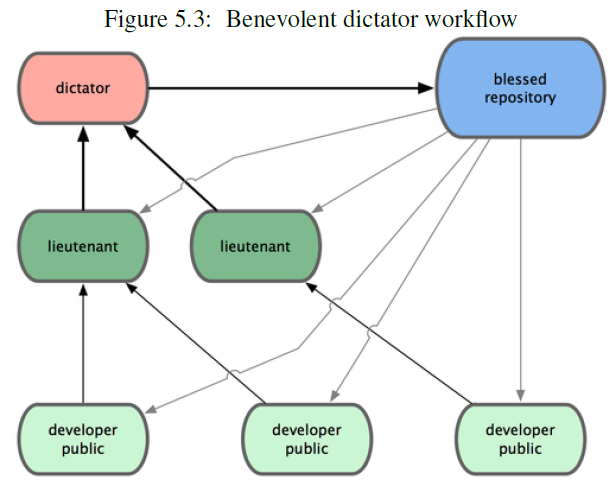
\includegraphics[scale=0.85]{figures/federatedGit.png}
	\caption[A distributed workflow to control for volatile versioning behavior.]{A distributed workflow to control for volatile versioning behavior.  From  \cite{cederqvist2002version}.}
	\label{fig:federated}
\end{figure}

\section{Change Logs} \label{sec:changelog}

Change logs, artifacts resulting from the versioning process, play a major role filling in gaps between versions.
They document changes and explain, in human language, the motivations behind these modifications \cite{uel1037}.
Since identifiers denote that a change has occurred, the logs provide details on how the changes modify an object's attributes.
They demonstrate a need and utility in understanding the deeper content of change beyond knowing that an object did transform.
While some data sets will provide a change log, software projects have normalized their use in version release documentation.
As a result, these projects provide a basis for understanding the value these logs can supply data sets with multiple versions.
The change log's common drawback is the limitation to only human readable text.
Wider adoption among data sets may be possible by making these texts machine computable.

Open source projects use change logs more consistently than data projects, which usually sport only use documentation.
Logs play an important communication role in these projects since developers can contribute without having been part of the original development team.
They allow developers to link bugs and errors with their corrections in new versions of the code \cite{Chen:2004:OCL:990374.990391}.
This gives insight into motivations behind particular design decisions.
It also provides feedback to the user community that corrections have been addressed, in addition to ensuring that improvements drive modifications to the code base.
An identifier cannot communicate these qualities while remaining succinct.
Some research has been done to determine the health of a development project based on the number and length of change logs released over time \cite{German03automatingthe}.
This becomes particularly significant as data freshness plays a growing role in successful system function \cite{Bouzeghoub:2004:FAD:1012453.1012464}.
However, little work has been done to make change logs machine-computable, as many of these documents remain in human-readable text only.
Research done involving change log content must manually link entries with computable meta-data such as the introduction of new features with the emergence of new bugs \cite{6132954}.
While machines may still be significantly removed from the ability to comprehend the impact of changes made to a data set or software code, they are currently opaquely blocked from consuming any of the content within logs more than understanding they contain text.
The transition between different versions of large data sets is then left largely up to the human user's ability to understand and process the modifications mentioned within the change log.

\subsection{Structured Data}

The Resource Description Framework in Attributes (RDFa) framework encodes linked data vocabularies into HTML documents, and provides an opportunity to make change logs machine interpretable. \cite{Adida2015}.
Linked data technologies utilize web ontologies to standardize terms and semantics across domain applications.
Automated agents can reason over a graph formed by linking these terms.
Encoding HTML documents with linked data better unlocks the content stored within.
\begin{figure}
	\centering
	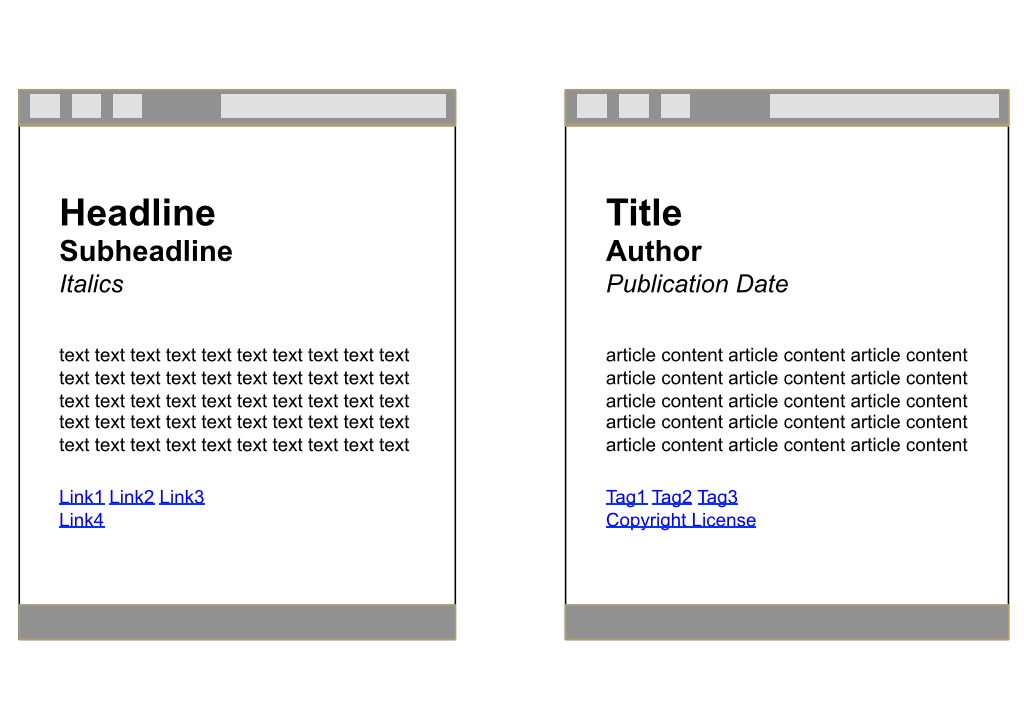
\includegraphics[scale=0.40]{figures/RDFaSemantics.png}
	\caption[Illustration of the difference in what autonomous systems see when crawling a web page and what humans see when reading the same material.]{Illustration of the difference in what autonomous systems see when crawling a web page and what humans see when reading the same material. Figure 1 from \cite{Herman2015}}
	\label{RDFa}
\end{figure}Figure \ref{RDFa} illustrates the semantic difference between what web crawlers and what humans see when they consume web pages.
People intuitively understand that certain strings represent meaningful information based on location and style.
RDFa seeks to encode that understanding natively for effective machine consumption.
Extending this approach into publishing change logs, will allow linked data to capture the metaphorical meat of change content.

The implementation requires changing publishing practices from plain-text documents to something structured-data compatible such as HTML.
The change also has the added benefit of making the logs available on-line, and thus, more openly accessible to data users through the utilization of web based search engines.
Large companies such as Google have already begun equipping their web crawlers to consume structured data such as RDFa from web pages.
RDFa has already had significant success in adoption across a variety of web publication platforms and eases the search for their content \cite{Bizer2013}.
However, the design of RDFa focuses on describing the web page's content through markup \cite{Herman2015}.
The underlying or resulting versioning data model may not conform with the format of content presented in the change log.
This would lead to a poorly structured graph or missing content, undermining the value gained by encoding linked data into the change log.
As a result, another method using JavaScript Object Notation for Linked Data (JSON-LD) was pursued since its purpose is to store data separate from visible content.

The JSON data format allows web pages to store data for JavaScript applications within the document.
It utilizes a simple and robust syntax to accommodate a wide variety of content.
JSON-LD extends the original specification by defining rules which allow entries to resolve as web vocabularies, giving them a meaningful context \cite{JSONLD}.
Because it stores data separate from visible content, JSON-LD does not need to adhere with the constraints of visible content.
However, every linked data triple must be explicitly defined, meaning that resulting documents may likely be much larger than their RDFa counterparts.

\section{Change Distance}

\subsection{Provenance Distance}

With increasing complexity, data workflows have developed in such a way that even subtle changes have serious implications for other parts of the workflow \cite{TILMES2011548}.
This observation makes change impact difficult to measure, but one insight begins with provenance's role in workflows.
Provenance can give great insight into a data object's future performance such as the  ability to predict disk usage based on the lineage of a data object \cite{dai2014provenance}.
Efforts have also been made to summarize provenance representations to improve consumption \cite{Ainy:2015:ASD:2806416.2806429}.
Changes to the process creating an object signals the development of a new version.
Therefore, studying the magnitude of this deviation should give some idea into the resulting object's impact.
This idea, known as provenance distance, seeks to determine the impact of changes in provenance on new data versions through measuring graph edit distances.

\begin{figure}
	\centering
	\begin{adjustbox}{addcode={\begin{minipage}{\width}}{
					\caption[Provenance graph of a Level 3 data product, showing the inter-relations between different data products in generating the final product.]{Provenance graph of a Level 3 data product, showing the inter-relations between different data products in generating the final product.  Figure 2 from \cite{TILMES2011548}}\end{minipage}},rotate=90,center}
		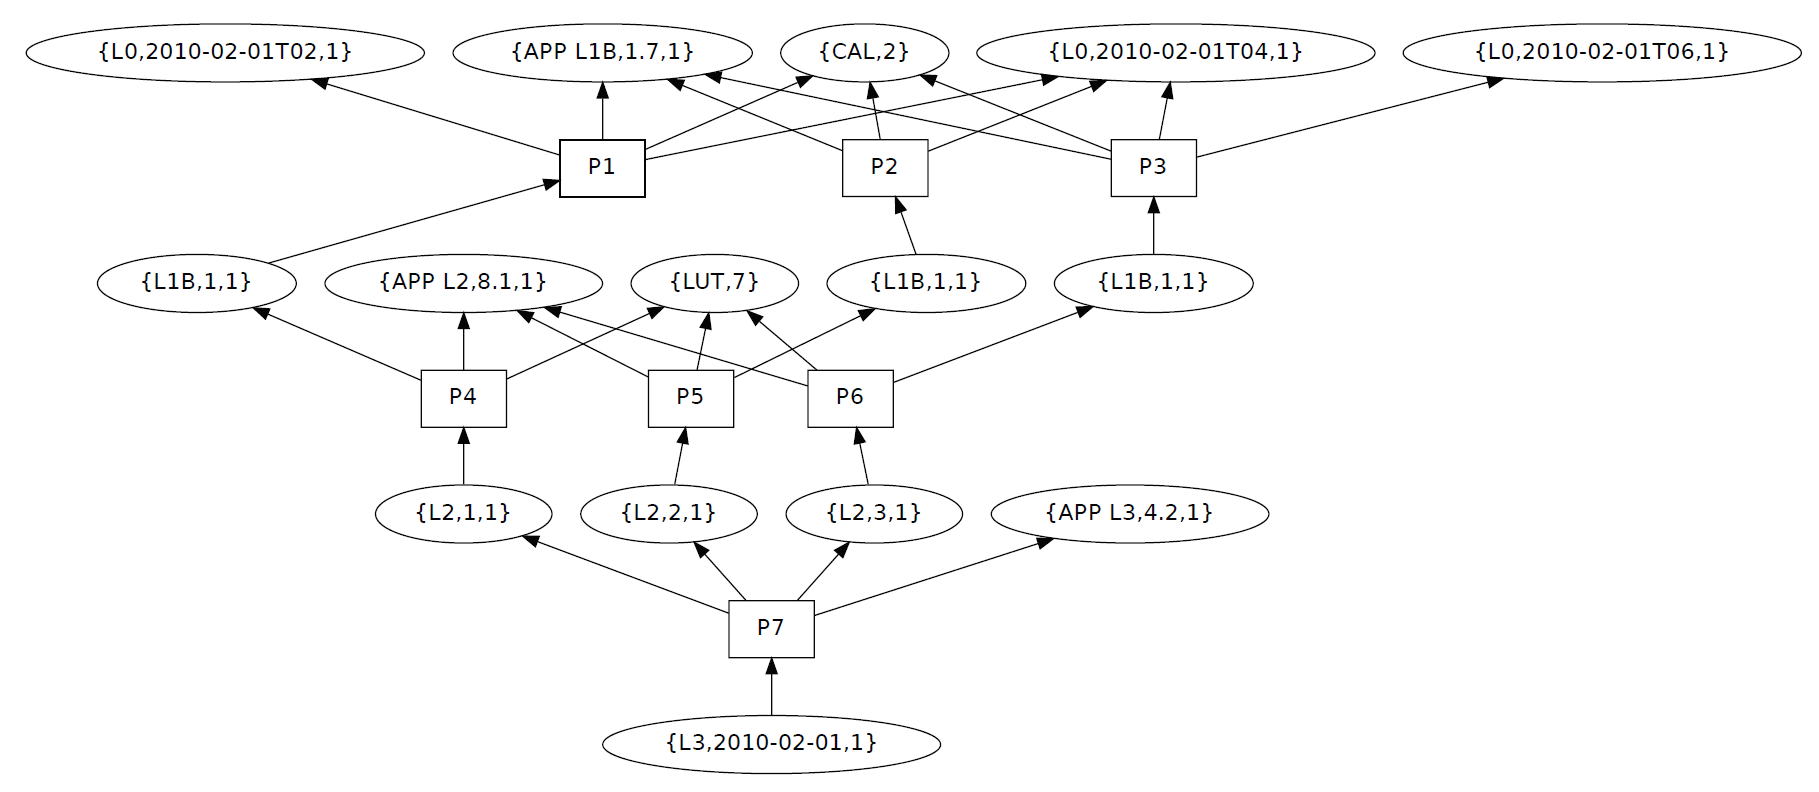
\includegraphics[scale=0.5]{figures/OzoneProvGraph.png}
	\end{adjustbox}
	\label{ProvGraph}
\end{figure}

The first ingredient necessary to calculate provenance distance is a linked data graph capturing the sequence of events leading to the old and new objects' creation, like the one shown in Figure \ref{ProvGraph}.
It shows the multiple lower level products involved in creating a Level 3 ozone indicator.
This can be accomplished through the use of previously mentioned provenance models, but these graphs are not widely available.
Using PROV to represent provenance data in a semantic model produces an acyclic directed graph with labeled nodes.
As a result, the provenance distance problem reduces to similarity measurement.
When calculating this measure, algorithms determine how far two graphs are from being isomorphic \cite{Cao2013}.
Node labeling simplifies this process by providing nodes which must match together, and greatly reduces the complexity from computing generalized graphs.
Graph Edit Distance, counting the edits necessary to transform one graph into another, provides a quantitative measure to associate with this process  \cite{Gao2010}.
Some variations count edge changes \cite{Goddard:1996:DGU:246962.246972}.

In Figure \ref{GraphEdit}, the left graph transforms through a move of edge 1 and a rotation of edge 4, resulting in an edit distance of two.
Such changes in a provenance graph would demonstrate an alteration in dependencies between objects used to generate a final notable product.
This kind of analysis resembles comparison measures employed in determining semantic similarity \cite{Hliaoutakis06informationretrieval}.
However, isolating changes responsible for differences in provenance can become difficult in complex environments as Tilmes observes in 2011, 
\begin{quotation}
	Consider the relatively common case of the calibration table, which is an input to the L1B process, changing. Even though the version of the L2 or L3 software hasn't changed, the data files in the whole process have been affected by the change in the calibration.
\end{quotation} \cite{TILMES2011548}.
L-number is shorthand for the level system featured in Figure \ref{NASALevels}.
While provenance distance may be straight-forward to calculate, the indicator hides many insights into an object's behavior.

\begin{figure}
	\centering
	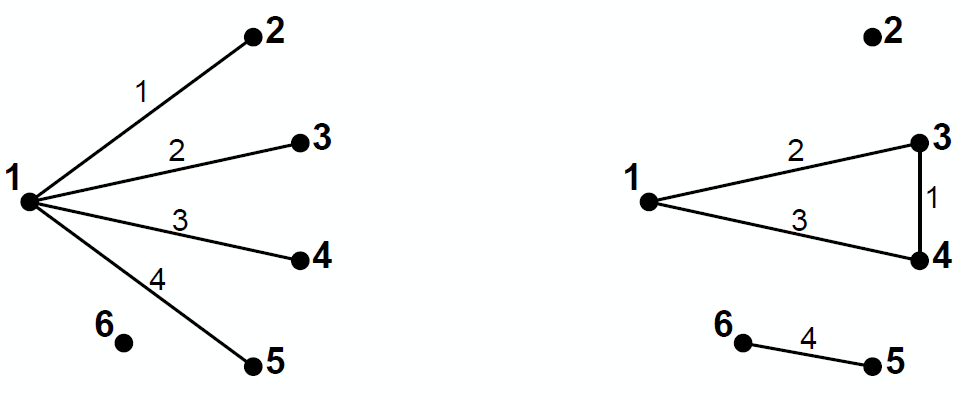
\includegraphics[scale=0.40]{figures/GraphEdit.png}
	\caption[The labeled graph on the left transforms into the right graph under two edge edits.]{The labeled graph on the left transforms into the right graph under two edge edits. Figure 2 from \cite{Goddard:1996:DGU:246962.246972}}
	\label{GraphEdit}
\end{figure}

Methods to provide quality of service boundaries leveraging provenance already exist which compare workflows based on performance criteria \cite{2015:CAA:2778374.2778504}.
However, these procedures focus primarily on quick retrieval and efficient storage instead of capitalizing on the latent information accessed by reasoning across data set versions \cite{tan2004research}.
The distance measures previously mentioned rely solely on provenance graphs to compute results, but this is obviously insufficient.
When considering the provenance of a data object, methods only consider the activities and entities that took an active role in the production of it.
A new version of an object has a familial relationship with its previous versions, but in most cases, they do not take an active role in its generation.
Without detailed change information, determining the difference between two data objects in a metric beyond broad strokes becomes difficult, if not impossible.

As per our definition of `version', objects must have common provenance, and the more similar they are, the more meaningful the results from versioning methods.
Provenance distance provides a means of determining how reliable versioning results are given a greater adoption of provenance graphs.
Measuring a change's impact with accuracy comparable to a change log requires a more detailed understanding and description than provenance can provide  \cite{Bose:2005:LRS:1057977.1057978}.
Sufficiently precise versioning measurements cannot be provided by provenance distance, but it could indicate the confidence of versioning results, which is out of scope for this project.

\section{Mapping}

Data managers primarily use one of two methods to store data versions: snapshots and deltas.
The snapshot method makes periodic copies of the data's state at a point in time.
While storing and retrieving these snapshots can be very quick, they require significant amounts of space to maintain.
The software manager GIT employs this method and Figure \ref{GITFile} demonstrates an example storage space for multiple versions \cite{Chacon:2009:PG:1618548}.
The squares with dotted outlines indicate unmodified files, which the system stores as pointers instead of full objects.
In addition, GIT compresses and separately stores very old versions which are unlikely to be accessed.
This versioning style may not be ideal for larger or often modified data sets as the size requirements will quickly grow unmanageable.
However, for many library or catalog environments, they cannot predict the target volume a user desires and must prioritize availability \cite{Payette2002} \cite{Barkstrom_digitallibrary}.
Some methods like the inverted file index have been developed to balance space and retrieval performance on web documents, especially since wikis and news feeds have grown in deployment \cite{Berberich:2007:TMT:1277741.1277831}.
Searches over these text media may require execution on older archived web pages.

\begin{figure}
	\centering
	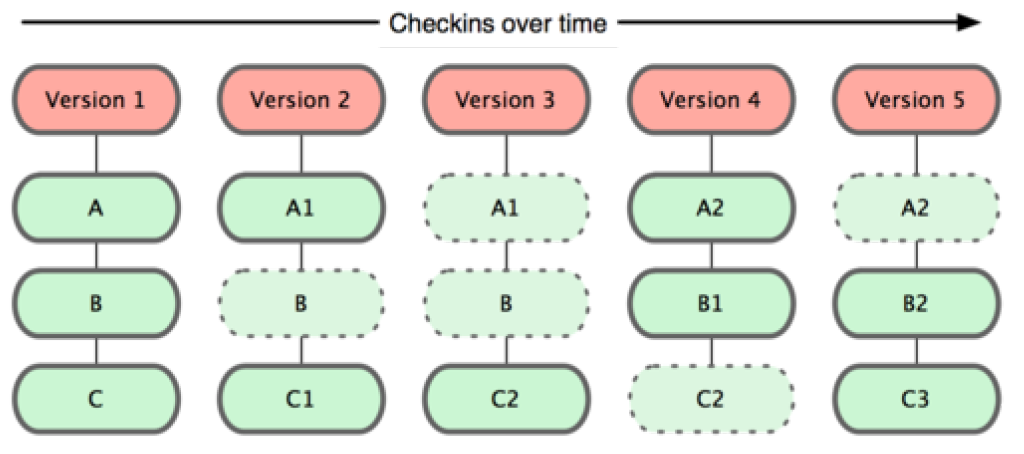
\includegraphics[scale=0.50]{figures/GITFiles.png}
	\caption[GIT stores changes in the repository as snapshots of individual files.]{GIT stores changes in the repository as snapshots of individual files. Figure 1.5 from \cite{Chacon:2009:PG:1618548}}
	\label{GITFile}
\end{figure}

The delta method entails calculating and storing only the differences between one version and the next.
Back delta variations store a snapshot of the most recent version and compute deltas towards older releases.
The forward delta variation stores the oldest data's snapshot and has deltas going forwards.
This method uses the minimum amount of space but trades it in for computation time to recreate any given version.
Particularly long running versioning systems occasionally save an intermittent snapshot to cut down on this processing time.
The setup proves ideal for data sets which prioritize service to their most recent versions \cite{Stuckenholz:2005:CEV:1039174.1039197}.
Because change documentation captures information between version objects, they most resemble differences calculated by the delta method.

Properly detecting changes in a system's files allows file managers to correctly group them into versions as seen in research conducted by the Atmospheric Radiation Measurements (ARM) group \cite{6906868}.
Difference or diff applications must first properly map data between objects and align them for comparison.
Many text-based data sets rely on well-established algorithms to perform this alignment  \cite{Chien:2000:VMX:646544.696357} \cite{Hartung201315}.
Sequential scientific data largely avoids this problem since developers already know the files or objects they replaced.
However, users do not have this advantage and system managers are starting to recognize the difference in versioning usage patterns between users and producers \cite{Branco2008}.
Mayernik, et al., probably gives the best description saying, "Prospective records document a process that must be followed to generate a given class of products whereas retrospective records document a process that has already been executed" \cite{MatthewS.Mayernik201312-039}.
While producers take a retrospective approach to version usage, consumers of new versions must take a prospective view, adapting to new changes.
This indicates that the orientation of versioning information reflects the imagined customer of that data.

Current linked data methods lack the fidelity to capture change information.
PROV and OPM express version changes as a single link, but capturing individual changes provides better detail, allowing more accurate distance measures.
Measuring change this way better communicates the change existing within a versioning system than courser methods leveraging only provenance graphs.
Implementing the version capture requires the procedures used to perform difference calculations and going a step further by creating linked data statements.
The model in Chapter \ref{ch:model} defines concepts to capture individual changes based on common operations and compares them with current methods of capture.

\section{Summary}
%%% Local Variables:
%%% mode: latex
%%% TeX-master: t
%%% End:
